\documentclass[11pt]{report}
\usepackage[letterpaper, total={6.5in, 10in}]{geometry}
%\usepackage{fancyhdr}
%\pagestyle{fancy}
\usepackage{amsmath, amsthm, mathpazo, epic, eepic, color, array}
\usepackage{amssymb}
%\usepackage{graphicx}
\usepackage{cancel}
\usepackage{pgfplots}
\usepackage{multicol}
\pgfplotsset{compat=1.13}
\usepackage{etoolbox}
\makeatletter
\patchcmd{\chapter}{\if@openright\cleardoublepage\else\clearpage\fi}{}{}{}
\makeatother
\usepackage{hyperref}

\usepackage{enumerate}
\usepackage{enumitem}

\usepackage{tikz}
\usetikzlibrary{positioning,chains,fit,shapes,calc,arrows,patterns}
\usepackage{tkz-graph}
\usetikzlibrary{arrows, petri, topaths}
\usepackage{tkz-berge}
\usepackage[all]{xy}
\usepackage{textcomp}
\usepackage{setspace}
\newlength\tindent
\setlength{\tindent}{\parindent}
\setlength{\parindent}{0pt}
\renewcommand{\indent}{\hspace*{\tindent}}

\newcommand{\ds}{\displaystyle}
\pgfplotsset{my style/.append style={axis x line=middle, axis y line=middle, xlabel={$x$}, ylabel={$y$}, axis equal }}




\begin{document}
\chapter{The Graphical Behavior of Functions}
%%%%%%%%%%%%%%%%%%%%%%%%%%%%Section 3.1%%%%%%%%%%%%%%%%%%%%%%%
\section{Extreme Values}

Write the definition of \textbf{absolute minimum}.
\vskip 1.5 in

Write the definition of \textbf{absolute maximum}.
\vskip 1.5 in

Collectively, the absolute minimum and absolute maximum are called \rule{4cm}{0.4pt}.\\ \\

Write the \textbf{Extreme Value Theorem}.
\vskip 1.5 in
\indent\textit{The Extreme Value Theorem guarantees that a continuous function on a closed interval will have a maximum and a minimum value.}\\
\newpage
Write the definition of \textbf{relative minimum}.
\vskip 1.5 in
Write the definition of \textbf{relative maximum}.
\vskip 1.5 in 
What is another name for a relative minimum? \rule{4cm}{0.4pt}\\ \\

\begin{multicols}{2}
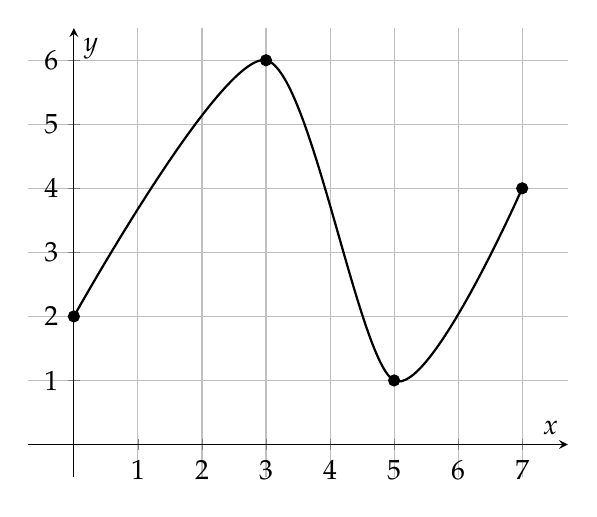
\begin{tikzpicture}
\begin{axis}[my style, ymajorgrids=true, xmajorgrids=true, xmin=-.5, xmax=7.5, ymin=-.5, ymax=6.5, xtick={1,2,3,4,5,6,7}, ytick={1,2,3,4,5,6}]
\addplot [thick,smooth] coordinates {(0,2)(3,6)(5,1)(7,4)};
\addplot[mark=*, only marks] coordinates {(3,6)(5,1)(0,2)(7,4)};
\end{axis}
\end{tikzpicture}\\


On the graph to the left:\\
\setstretch{1.6}{\indent What is the absolute minimum value of $f$?\rule{4cm}{0.4pt}\\
\indent What is the absolute minimum value of $f$? \rule{4cm}{0.4pt}\\
\indent Is (3,6) a relative maximum? \rule{4cm}{0.4pt}\\
\indent Is (5,1) a relative minimum? \rule{4cm}{0.4pt}\\
\indent Is (7,4) a relative maximum? \rule{4cm}{0.4pt} \\}

\end{multicols}

\newpage

Match the following statements with the correct graph below. \\
\indent On each graph CLEARLY label where the relative max, relative min, absolute max, and\\ \indent absolute min are, if applicable.\\
\indent \indent \textit{\textbf{Note:}} a point may be both a relative and absolute max or both a relative and absolute min!\\
\indent\indent\indent a) Graph has no absolute or relative extrema.\\
\indent\indent\indent b) Graph has relative max and min, but no absolute extrema.\\
\indent\indent\indent c) Graph has a relative max, relative min, absolute max, and absolute min.\\
\indent\indent\indent d) Graph has a relative min, absolute min, and absolute max.\\
\indent\indent\indent e) Graph has a relative and absolute min.\\ 
\indent\indent\indent f) Graph has a relative min, relative max, and absolute max.\\

\begin{multicols}{2}

\begin{tikzpicture}
\begin{axis}[my style, xmin=-3, xmax=3, ymin=-3, ymax=3, xtick={-3,-2,...,3}, ytick={-3,-2,...,3}]
\addplot[domain=-3:3,samples=100, smooth] {2*x^3-3*x^2-3*x+2};
\end{axis}
\end{tikzpicture}  \rule{.75cm}{0.4pt}

\begin{tikzpicture}
\begin{axis}[my style, xmin=-2, xmax=4, ymin=-5, ymax=5, xtick={-2,-1,...,4}, ytick={-3,-2,...,5}]
\addplot[domain=-2:4,samples=100, smooth] {.8*(x^4-5*x^3+5*x^2+3*x-3)};
\end{axis}
\end{tikzpicture} \rule{.75cm}{0.4pt}

\begin{tikzpicture}
\begin{axis}[my style, xmin=-2, xmax=2, ymin=-3, ymax=3, xtick={-3,-2,-1,...,2,3}, ytick={-3,-2,...,3}]
\addplot[domain=-1.35:1.15,samples=100, smooth] {-1*(2*x^3-x^2-2*x+2)};
\addplot[mark=*, only marks] coordinates {(-1.32,2)(1.13,-1.5)};
\end{axis}
\end{tikzpicture} \rule{.75cm}{0.4pt}

\begin{tikzpicture}
\begin{axis}[my style, xmin=-3, xmax=3, ymin=-3, ymax=3, xtick={-3,-2,-1,...,1,2,3}, ytick={-3,-2,...,3}]
\addplot[domain=-3:3, smooth] {3*x^2+3*x-2};
%\addplot[mark=*, only marks] coordinates {(3,6)(5,1)(0,2)(7,4)};
\end{axis}
\end{tikzpicture} \rule{.75cm}{0.4pt}

\begin{tikzpicture}
\begin{axis}[axis equal, axis x line=middle, axis y line=middle, xlabel={$x$}, ylabel={$y$}, xmin=-2.5, xmax=1.5, ymin=-3, ymax=3, xtick={-3,-2,-1,...,1,2}, ytick={-3,-2,...,3}]
\addplot[domain=-2:.5, smooth] {2*x^2+2*x-2};
\addplot[mark=*, only marks] coordinates {(-2,2)(.5,-.5)};
\end{axis}
\end{tikzpicture} \rule{.75cm}{0.4pt}

\begin{tikzpicture}
\begin{axis}[my style, xmin=-1, xmax=3, ymin=-3, ymax=3, xtick={-1,0,...,1,2,3}, ytick={-3,-2,...,3}]
\addplot[domain=-3:3, smooth] {(x-1.5)^3-.5};
\end{axis}
\end{tikzpicture} \rule{.75cm}{0.4pt}
\end{multicols}
\newpage

Write the definition of \textbf{critical number}.\\

\vskip 1 in

Find the critical numbers of $f(x)=x^3-6x^2-15x+7$

\vskip 1.5 in

Use \textbf{Key Idea 4} to find the extreme values of $f(x)=5+54x-2x^3$ on the interval $[0,4]$. Clearly show your work for each of the 4 steps given in Key Idea 4.

\vskip 2 in


\newpage


%%%%%%%%%%%%%%%%  Section 3.2%%%%%%%%%%%%%%%%%%%%%%%%%%%%%%%%%%%%%%

\section{The Mean Value Theorem}

Write the \textbf{Mean Value Theorem of Differentiation (MVT)}.\\
\indent Let $f$ be a function that satisfies the following conditions.
\begin{doublespacing}
\begin{enumerate}
\item
\item  
\end{enumerate}
\end{doublespacing}
Then
\vskip 1 in 

Write \textbf{Rolle's Theorem}.
\indent Let $f$ be a function that satisfies the following conditions.
\begin{doublespacing}
\begin{enumerate}
\item
\item  
\item
\end{enumerate}
\end{doublespacing}
Then
\vskip 1 in 

Compare \textbf{MVT} and \textbf{Rolle's Theorem}.\\
\indent  What is the same for each theorem?
\vskip 1 in
\indent How do the theorems differ?
\vskip 1 in
\indent What is the conclusion of the MVT if $f(a)=f(b)$?
\vskip 1 in



\begin{tikzpicture}
\begin{axis}[axis equal, axis x line=middle, axis y line=middle, xmin=-.2, xmax=2.2, ymin=-.2, ymax=1.5, xtick={.5, 1.1, 2}, ytick style={draw=none},yticklabels=empty, xticklabels={$a$, $c$, $b$},name=myplot]
\draw (.5,.3) .. controls (1,1.3) and (1.2,1.1) .. (2,.75);
\draw ( 2,1) node (b){\scriptsize $f(x)$};
\draw [black,->] (b)--(1.75,.9);
\draw(1.2,1.4) node (a) {\scriptsize{tangent line}};
\draw [{black},->] (a) -- (1.4,1.15);
\draw(1.4,.3) node (c) {\scriptsize{secant line}};
\draw[black,->] (c)--(1.3,.5); 
\addplot[mark=*, only marks] coordinates {(.5,.3)(2,.75)(1.1,1.02)};
\addplot[domain=.2:2.3, black, smooth] {.3*x+.15};
\addplot[domain=.2:2.3, black, dashed, smooth] {(.3*x+.15)+.54};
\draw[dashed, thin, red] (1.1,0)--(1.1,1.02);
%\draw (.5,.3) -- (2,.75);
\end{axis}
\node [right] at (myplot.right of origin) {\scriptsize $x$};
\node [above] at (myplot.above origin) {\scriptsize $y$};
\end{tikzpicture}

In your own words, use the graph above to explain the Mean Value Theorem.\\





 I made a pretty graph so I want to use it!!! Is the above question good enough?\\
Should we be asking questions about the videos?

\newpage
 
%%%%%%%%%%%%%%%%%   Section 3.3  %%%%%%%%%%%%%%%%%%%%%%%%%%%%%%%

\section{Increasing and Decreasing Functions}

Write the definition of \textbf{increasing function}.
\vskip 1.25 in
Write the definition of \textbf{decreasing function}.
\vskip 1.25 in

Write the \textbf{Test for Increasing/Decreasing Functions}.
\vskip 1.75 in

Graph the functions $f(x)=(x-1)^2+2$ and $f'(x)=2(x-1)=2x-2$ on the axes below.
\begin{multicols}{2}
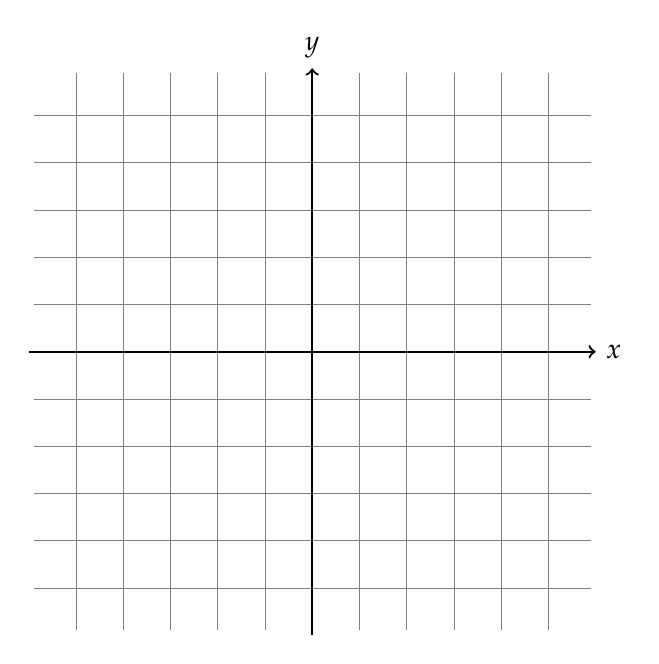
\begin{tikzpicture}[scale=.6]
\draw[help lines, color=gray] (-5.9,-5.9) grid (5.9,5.9);
\draw[->,thick] (-6,0)--(6,0) node[right]{$x$};
\draw[->,thick] (0,-6)--(0,6) node[above]{$y$};
\end{tikzpicture}
\begin{enumerate}
\begin{doublespacing}
\item On what interval is $f(x)$ increasing? \rule{.75cm}{0.4pt}
\item On what interval is $f'(x)>0$? \rule{.75cm}{0.4pt}
\item On what interval is $f(x)$ decreasing? \rule{.75cm}{0.4pt}
\item On what interval is $f'(x)<0$? \rule{.75cm}{0.4pt}
\end{doublespacing}
\item Do your results from 1-4 support or conflict with the Test for Increasing/Decreasing Functions? Explain.
\end{enumerate} 
\end{multicols}

\newpage

State the \textbf{First Derivative Test}. \vskip 2 in

Look at your graph of $f(x)=(x-2)^2+2$ and $f'(x)=2(x-1)=2x-2$ on the previous page.
\begin{enumerate}
\item At what $x$ value does $f'(x)$ change signs?\rule{4 cm}{.4pt}
\item Does the function $f(x)$ have a relative maximum or minimum at this value?\rule{4 cm}{.4pt}
\end{enumerate}

\vskip .25 in
Complete the following steps to find the intervals on which $f(x)=x\sqrt{6-x}$ is increasing or decreasing.
\begin{enumerate}
\item Find the critical numbers of $f$.
\begin{enumerate}
\item
To do this, determine where $f'(x)=0$ or is undefined.
\item Show your work to find $\displaystyle f'(x)=\frac{-3x+12}{2\sqrt{6-x}}$.
\vskip 2 in
\item The critical number(s) of $f$ are \rule{4 cm}{.4pt}
\end{enumerate}
\item Split the domain of $f$, which is $(-\infty, 6]$, into intervals using the critical numbers of $f$.
\begin{center}
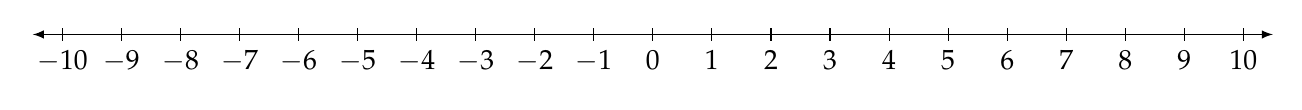
\begin{tikzpicture}[scale=.75]
\draw[latex-latex] (-10.5,0) -- (10.5,0) ; %edit here for the axis
\foreach \x in  {-10,-9, ...,8,9,10} % edit here for the vertical lines
\draw[shift={(\x,0)},color=black] (0pt,3pt) -- (0pt,-3pt);
\foreach \x in  {-10,-9, ...,8,9,10} % edit here for the numbers
\draw[shift={(\x,0)},color=black] (0pt,0pt) -- (0pt,-3pt) node[below] 
{$\x$};
\end{tikzpicture}
\end{center}
\item Determine the sign of $f'$ in each of the intervals above.\\
\indent \textit{NOTE:} You should have OPEN intervals in each case.\\ \indent $f$ will not be increasing or decreasing when $f'$ is 0 or at an endpoint of the domain.

\begin{center}
\bgroup
\def\arraystretch{2.1}
\begin{tabular}{|m{4cm}|m{3cm} |m{3 cm}|}
\hline
\textbf{Interval} & \textbf{Sign of $f'$} &\textbf{Behavior of $f$}\\
\hline
  & & \\
\hline
 & &\\
\hline
\end{tabular}
\egroup
\end{center}
\vskip .25 in
\item $f$ is increasing on \rule{4 cm}{.4 pt} and $f$ is decreasing on \rule{4 cm}{.4 pt}.
\vskip .25 in
\item Use the First Derivative Test and the information above to determine where $f$ has a relative maximum or a relative minimum if applicable.
\end{enumerate}

\newpage


%%%%%%%%%%%%%%%%%% Section 3.4 %%%%%%%%%%%%%%%%%%%%%%%%%
\section{Concavity and the Second Derivative}

State the definition of \textbf{Concave Up and Concave Down}.
\vskip 1 in
Geometrically, what does it mean when a function is 
\begin{enumerate}
\begin{doublespacing}
\item concave up?\rule{12 cm}{.4pt}
\item concave down?\rule{11.5 cm}{.4pt}
\end{doublespacing}
\end{enumerate}

State the \textbf{Test for Concavity}.
\vskip 1.5 in

State the definition of \textbf{point of inflection}.
\vskip 1 in

Draw a curve that satisfies the following requirements.
\begin{multicols}{2}
\begin{center}
\bgroup
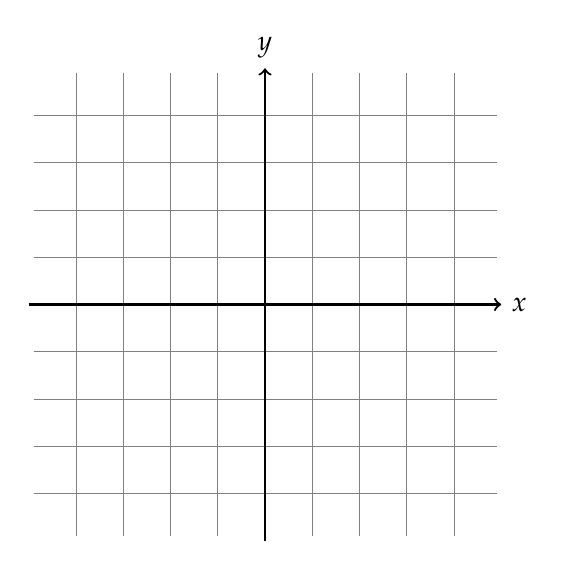
\begin{tikzpicture}[scale=.6]
\draw[help lines, color=gray] (-4.9,-4.9) grid (4.9,4.9);
\draw[->,thick] (-5,0)--(5,0) node[right]{$x$};
\draw[->,thick] (0,-5)--(0,5) node[above]{$y$};
\end{tikzpicture}\\
Concave upward and decreasing\\
\egroup
\end{center}
\begin{center}
\bgroup
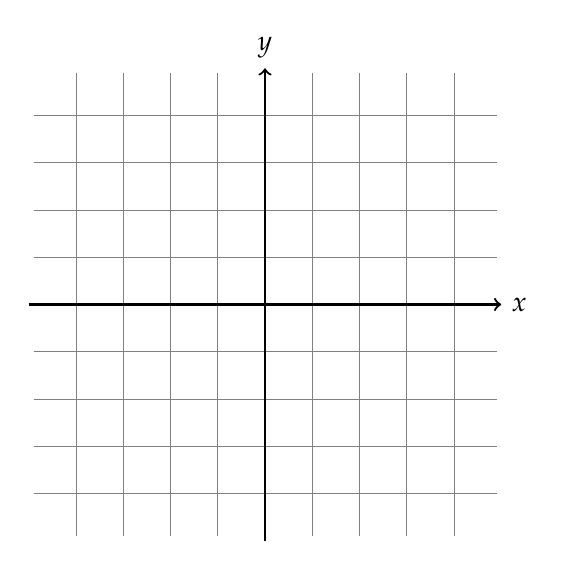
\begin{tikzpicture}[scale=.6]
\draw[help lines, color=gray] (-4.9,-4.9) grid (4.9,4.9);
\draw[->,thick] (-5,0)--(5,0) node[right]{$x$};
\draw[->,thick] (0,-5)--(0,5) node[above]{$y$};
\end{tikzpicture}\\
Concave upward and increasing\\
\egroup
\end{center}
\begin{center}
\bgroup
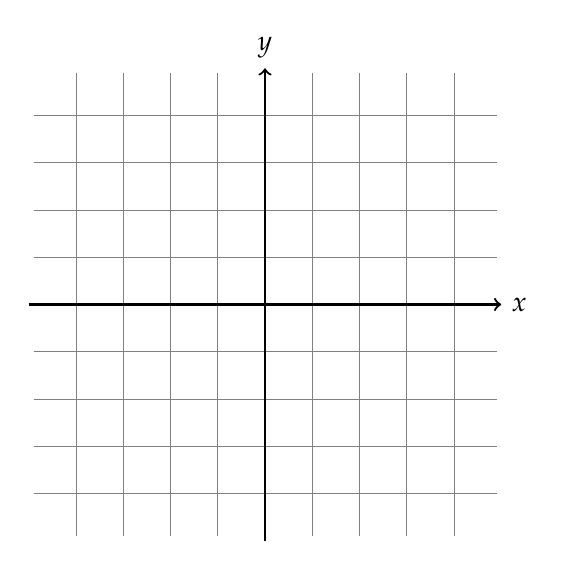
\begin{tikzpicture}[scale=.6]
\draw[help lines, color=gray] (-4.9,-4.9) grid (4.9,4.9);
\draw[->,thick] (-5,0)--(5,0) node[right]{$x$};
\draw[->,thick] (0,-5)--(0,5) node[above]{$y$};
\end{tikzpicture}\\
Concave downward and decreasing\\
\egroup
\end{center}
\begin{center}
\bgroup
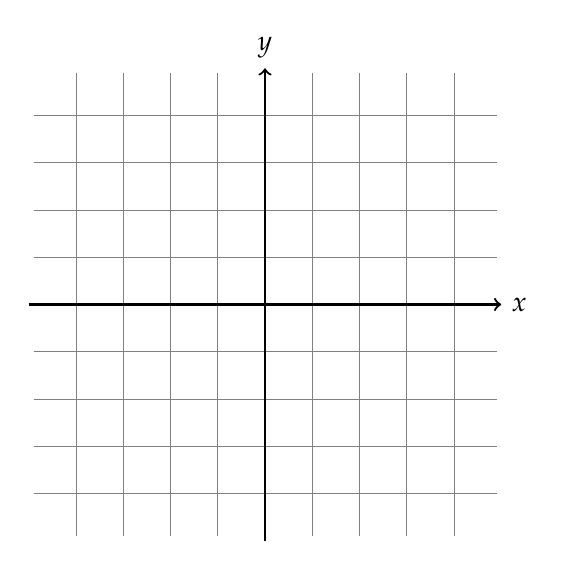
\begin{tikzpicture}[scale=.6]
\draw[help lines, color=gray] (-4.9,-4.9) grid (4.9,4.9);
\draw[->,thick] (-5,0)--(5,0) node[right]{$x$};
\draw[->,thick] (0,-5)--(0,5) node[above]{$y$};
\end{tikzpicture}\\
Concave downward and increasing
\egroup
\end{center}
\end{multicols}

Complete the following steps to determine the intervals on which $\ds f(x)=\frac{x}{x^2+1}$ is concave up and concave down.
\begin{enumerate}
\item Determine where $f''(x)$ is 0 or undefined.\\
\indent Show your work to find $\ds f''(x)=\frac{2x(x^2-3)}{(x^2+1)^3}$.
\vskip 3 in
\item Use the values from 1. to split the domain of $f(x)$, which is $(-\infty,\infty )$.
\begin{center}
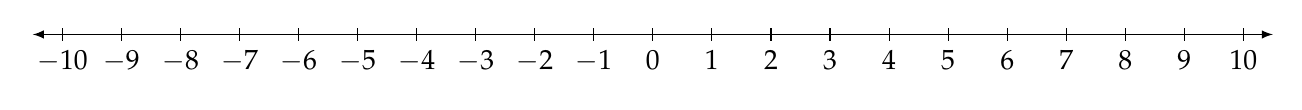
\begin{tikzpicture}[scale=.75]
\draw[latex-latex] (-10.5,0) -- (10.5,0) ; %edit here for the axis
\foreach \x in  {-10,-9, ...,8,9,10} % edit here for the vertical lines
\draw[shift={(\x,0)},color=black] (0pt,3pt) -- (0pt,-3pt);
\foreach \x in  {-10,-9, ...,8,9,10} % edit here for the numbers
\draw[shift={(\x,0)},color=black] (0pt,0pt) -- (0pt,-3pt) node[below] 
{$\x$};
\end{tikzpicture}
\end{center}
\item Determine the sign of $f''(x)$ in each of the intervals.
\begin{center}
\bgroup
\def\arraystretch{2.1}
\begin{tabular}{|m{4cm}|m{3cm} |m{3 cm}|}
\hline
\textbf{Interval} & \textbf{Sign of $f''$} &\textbf{Behavior of $f$}\\
\hline
  & & \\
\hline
 & &\\
\hline
\end{tabular}
\egroup
\end{center}
\vskip .25 in
\item $f$ is concave up on \rule{4 cm}{.4 pt} and $f$ is concave down on \rule{4 cm}{.4 pt}.
\vskip .25 in
\item Determine if $f(x)$ has any inflection points and if applicable find them.
\vskip .5 in
\end{enumerate}

State the \textbf{Second Derivative Test}.
\vskip 2 in

Should we have an example here?\\
Nothing in book about test failing when $f''(x)=0$

\newpage

%%%%%%%%%%%%%%%%%%% Section 3.5  %%%%%%%%%%%%%%%%%%%%%%%%%%%

\section{Curve Sketching}

Read through the curve sketching guidelines given in \textbf{Key Idea 7} and \textbf{Examples 1-3}. Complete the following problem.

We will complete the steps to graph $\mathbf{\ds f(x)=\frac{x^2-1}{x^2-9}}$.
\begin{enumerate}
\item Find the domain of $f(x)$.
\vskip .75 in
\item Find any vertical asymptotes.
\begin{enumerate}
\item $\ds f(x)=\frac{x^2-1}{x^2-9}$ has vertical asymptotes at $x=3$ and $x=-3$.
\item Show the appropriate limits to verify the vertical asymptotes. You should show four limits.
\vskip 2 in
\end{enumerate}
\item Find the $x$ and $y$ intercepts of $f$ and any symmetry.
\begin{enumerate}
\item Find the $x$-intercept.
\vskip .5 in
\item Find the $y$-intercept.
\vskip .5 in
\item Determine if there is any symmetry.\\
\indent Remember: $f(x)$ is even and has $y$-axis symmetry if $f(-x)=f(x)$.\\
\indent $f(x)$ is odd and has origin symmetry if $f(-x)=-f(x)$.
\vskip 1 in
\end{enumerate}
\item Determine the limits $\ds \lim_{x\to -\infty} f(x)$ and $\ds \lim_{x\to \infty} f(x)$.\\
\indent Does $f(x)$ have any horizontal asymptotes? If so, clearly state the horizontal asymptote.  \rule{4 cm}{.4 pt}
\vskip 1.5 in
\item Find the critical values of $f(x)$.
\begin{enumerate}
\item Show your work to find $\ds f'(x)=\frac{-16x}{(x^2-9)^2}$.
\vskip 2 in
\item The critical values of $f(x)$ are  \rule{4 cm}{.4 pt}.
\end{enumerate}
\item Find the possible points of inflection of $f(x)$.
\begin{enumerate}
\item Show your work to find $\ds f''(x)=\frac{48x^2+144}{(x^2-9)^3}$.
\vskip 2 in
\item Possible $x$ value(s) for points of inflection are  \rule{4 cm}{.4 pt}.
\end{enumerate}
\item 
Determine where $f(x)$ is increasing, decreasing, concave up and concave down. Complete the chart as in Examples 1-3.
\begin{center}
\setlength{\unitlength}{4.6em}
\begin{picture}(6,2)
\scriptsize
\put(.4,0){\line(0,1){1.6}}
\multiput(1.7,.5)(1.4,0){3}{\line(0,1){1.1}}
%\multiput(.7,1.44)(.5,0){9}{\line(0,1){.1}}
\put(.8,1.44){\line(0,1){.1}}
\put(1.25,1.44){\line(0,1){.1}}
\put(2.15,1.44){\line(0,1){.1}}
\put(2.65,1.44){\line(0,1){.1}}
\put(3.5,1.44){\line(0,1){.1}}
\put(4,1.44){\line(0,1){.1}}
\put(5,1.44){\line(0,1){.1}}
\multiput(0,.5)(0,.5){2}{\line(1,0){5.5}}
\put(2.5,1.5){\vector(1,0){3}}
\put(2.5,1.5){\vector(-1,0){2.5}}
\put(-.1,1.45){$x$}
\put(1.55,1.65){$-3$}
\put(3.05,1.65){$0$}
\put(4.45,1.65){$3$}
%\put(4.1,1.65){$0$}
%\put(4.95,1.65){$1.064$}
\put(.1,1.1){$f'$}
\put(.1,.6){$f''$}
\put(.1,.1){$f$}
\put(1.5,.1) {\scriptsize{undef}}
\put(4.4,.1) {\scriptsize{undef}}
\put(3,.1) {$\frac19$}
\end{picture}
\end{center}	

\item
Sketch the graph.
\begin{center}
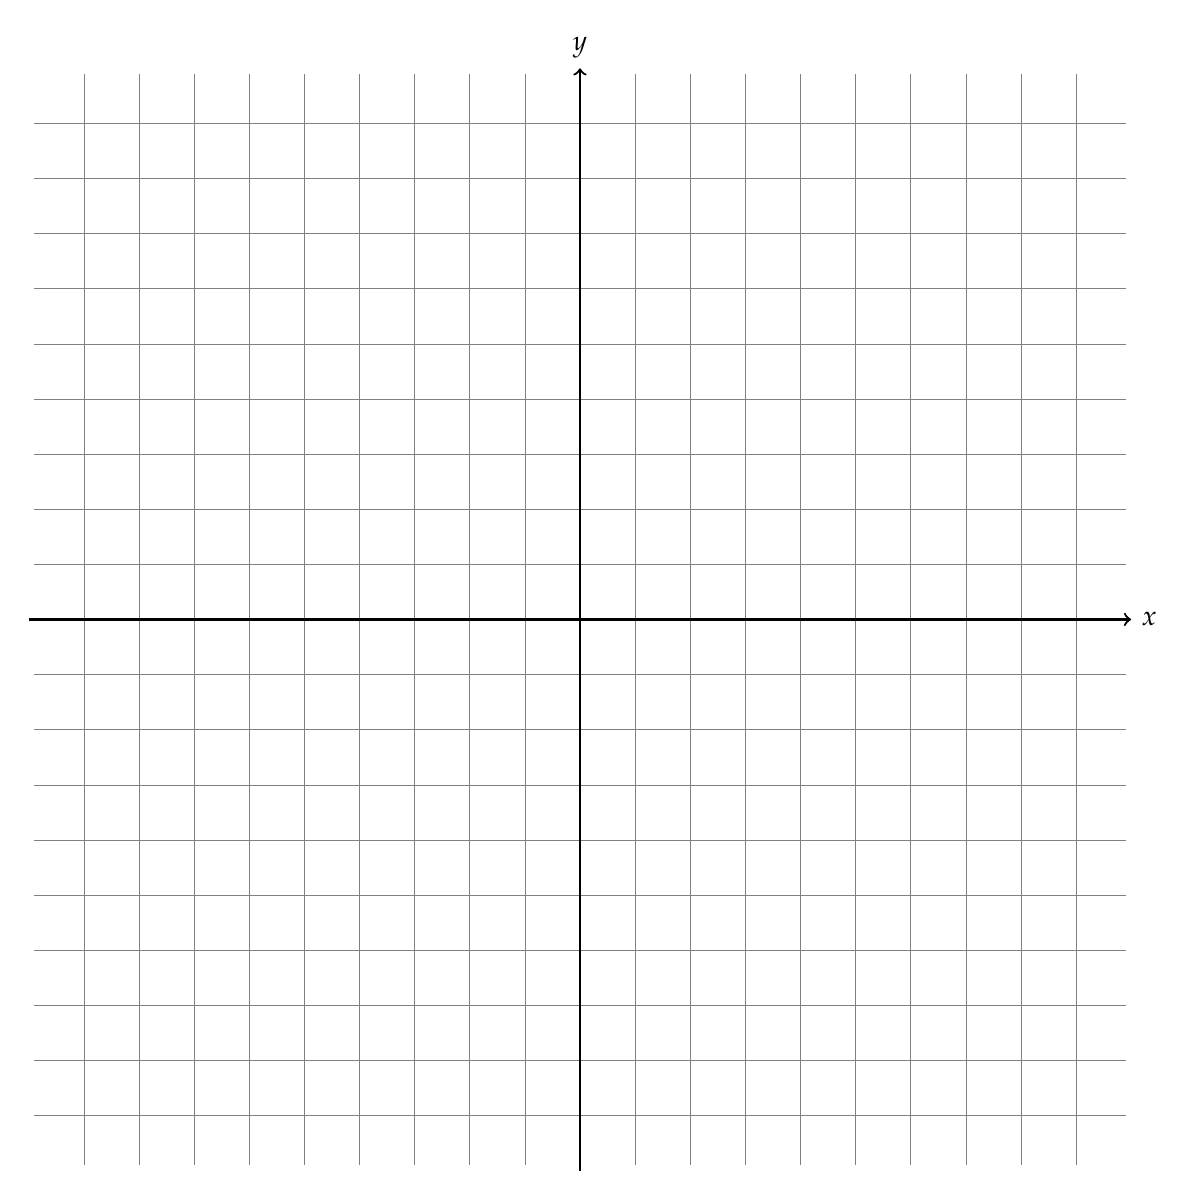
\begin{tikzpicture}[scale=.7]
\draw[help lines, color=gray] (-9.9,-9.9) grid (9.9,9.9);
\draw[->,thick] (-10,0)--(10,0) node[right]{$x$};
\draw[->,thick] (0,-10)--(0,10) node[above]{$y$};
\end{tikzpicture}
\end{center}
\end{enumerate}

\end{document}